%Version 3.1 December 2024
% See section 11 of the User Manual for version history
%
%%%%%%%%%%%%%%%%%%%%%%%%%%%%%%%%%%%%%%%%%%%%%%%%%%%%%%%%%%%%%%%%%%%%%%
%%                                                                 %%
%% Please do not use \input{...} to include other tex files.       %%
%% Submit your LaTeX manuscript as one .tex document.              %%
%%                                                                 %%
%% All additional figures and files should be attached             %%
%% separately and not embedded in the \TeX\ document itself.       %%
%%                                                                 %%
%%%%%%%%%%%%%%%%%%%%%%%%%%%%%%%%%%%%%%%%%%%%%%%%%%%%%%%%%%%%%%%%%%%%%

%%\documentclass[referee,sn-basic]{sn-jnl}% referee option is meant for double line spacing

%%=======================================================%%
%% to print line numbers in the margin use lineno option %%
%%=======================================================%%

%%\documentclass[lineno,pdflatex,sn-basic]{sn-jnl}% Basic Springer Nature Reference Style/Chemistry Reference Style

%%=========================================================================================%%
%% the documentclass is set to pdflatex as default. You can delete it if not appropriate.  %%
%%=========================================================================================%%

%%\documentclass[sn-basic]{sn-jnl}% Basic Springer Nature Reference Style/Chemistry Reference Style

%%Note: the following reference styles support Namedate and Numbered referencing. By default the style follows the most common style. To switch between the options you can add or remove “Numbered” in the optional parenthesis. 
%%The option is available for: sn-basic.bst, sn-chicago.bst%  
 
%%\documentclass[pdflatex,sn-nature]{sn-jnl}% Style for submissions to Nature Portfolio journals
%%\documentclass[pdflatex,sn-basic]{sn-jnl}% Basic Springer Nature Reference Style/Chemistry Reference Style
\documentclass[pdflatex,sn-mathphys-num]{sn-jnl}% Math and Physical Sciences Numbered Reference Style
%%\documentclass[pdflatex,sn-mathphys-ay]{sn-jnl}% Math and Physical Sciences Author Year Reference Style
%%\documentclass[pdflatex,sn-aps]{sn-jnl}% American Physical Society (APS) Reference Style
%%\documentclass[pdflatex,sn-vancouver-num]{sn-jnl}% Vancouver Numbered Reference Style
%%\documentclass[pdflatex,sn-vancouver-ay]{sn-jnl}% Vancouver Author Year Reference Style
%%\documentclass[pdflatex,sn-apa]{sn-jnl}% APA Reference Style
%%\documentclass[pdflatex,sn-chicago]{sn-jnl}% Chicago-based Humanities Reference Style

%%%% Standard Packages
%%<additional latex packages if required can be included here>

\usepackage{graphicx}%
\usepackage{multirow}%
\usepackage{amsmath,amssymb,amsfonts}%
\usepackage{amsthm}%
\usepackage{mathrsfs}%
\usepackage[title]{appendix}%
\usepackage{xcolor}%
\usepackage{textcomp}%
\usepackage{manyfoot}%
\usepackage{booktabs}%
\usepackage{algorithm}%
\usepackage{algorithmicx}%
\usepackage{algpseudocode}%
\usepackage{listings}%
\usepackage{float}
%%%%

%%%%%=============================================================================%%%%
%%%%  Remarks: This template is provided to aid authors with the preparation
%%%%  of original research articles intended for submission to journals published 
%%%%  by Springer Nature. The guidance has been prepared in partnership with 
%%%%  production teams to conform to Springer Nature technical requirements. 
%%%%  Editorial and presentation requirements differ among journal portfolios and 
%%%%  research disciplines. You may find sections in this template are irrelevant 
%%%%  to your work and are empowered to omit any such section if allowed by the 
%%%%  journal you intend to submit to. The submission guidelines and policies 
%%%%  of the journal take precedence. A detailed User Manual is available in the 
%%%%  template package for technical guidance.
%%%%%=============================================================================%%%%

%% as per the requirement new theorem styles can be included as shown below
\theoremstyle{thmstyleone}%
\newtheorem{theorem}{Theorem}%  meant for continuous numbers
%%\newtheorem{theorem}{Theorem}[section]% meant for sectionwise numbers
%% optional argument [theorem] produces theorem numbering sequence instead of independent numbers for Proposition
\newtheorem{proposition}[theorem]{Proposition}% 
%%\newtheorem{proposition}{Proposition}% to get separate numbers for theorem and proposition etc.

\theoremstyle{thmstyletwo}%
\newtheorem{example}{Example}%
\newtheorem{remark}{Remark}%

\theoremstyle{thmstylethree}%
\newtheorem{definition}{Definition}%

\raggedbottom
%%\unnumbered% uncomment this for unnumbered level heads

\begin{document}



%%=============================================================%%
%%
%%                    BEGINNING OF PAPER
%%
%%=============================================================%%



\title[Tennis Action Recognition with Tao Toolkit]{Tennis Action Recognition with Tao Toolkit}

\author{\fnm{Gary} \sur{Wang}}\email{dwang3@oxy.edu}
\author{\fnm{Max} \sur{Tulley}}\email{tulley@oxy.edu}


%%=============================================================%%
%% ABSTRACT + KEYWORDS
%%=============================================================%%


\abstract{The process of recognizing and labeling actions in the context of tennis is a challenging task for lightweight models. Tennis actions are not only composed of fine and subtle movements that are difficult to distinguish, but also often require surrounding context to be correctly labeled, for example, a serve and a smash can appear very similar when the ball or full scene is not visible. In this project, we attempt to address this task by utilizing the NVIDIA TAO Toolkit and its DeepStream pipelines to train models to recognize tennis actions and perform real-time continuous inference on a live video feed. Although training results were promising, actual field testing was disappointing. Additionally, our work is constrained by the limited availability of data, as we rely on a relatively small and outdated dataset.
}

\keywords{Action Recognition, Tennis, Deep Learning, Pose Estimation, Graph Convolutional Networks, NVIDIA TAO Toolkit, DeepStream, Transfer Learning, Skeleton-Based Classification, Sports Analytics}

\maketitle


%%=============================================================%%
%% INTRODUCTION
%%=============================================================%%


\section{Introduction}\label{sec1}


Although the task of recognizing tennis poses from video may initially seem narrow, the ability to accurately classify human actions is a fundamental problem in computer vision with wide ranging applications. Beyond sports analytics where athletes can use such systems to improve technique action recognition models have uses in public safety for example detecting dangerous behavior, interactive systems such as video games, and even military and surveillance contexts.

In this project, we investigate whether lightweight action recognition models can effectively handle complex tasks such as tennis action classification. Specifically, we aim to answer two research questions --- whether lightweight models that can be trained using the NVIDIA TAO Toolkit are capable of achieving strong performance on action recognition tasks, and whether these models can perform real time inference when deployed using the DeepStream pipeline.

We focus primarily on two pipelines in the TAO toolkit --- ActionRecognitionNet3D which is an end to end pipeline which takes as input video frames and outputs the class label and BodyPose3DNet in combination with PoseClassificationNet. 

We hypothesize that models trained within the TAO Toolkit can achieve acceptable accuracy in tennis action recognition despite the difficulty of the task \cite{thetis}, and that their lightweight design enables efficient real time inference when integrated into a streaming pipeline.


%%=============================================================%%
%% RELATED WORKS
%%=============================================================%%


\section{Related Works}\label{sec2}


\subsection{THETIS Dataset}

The THETIS Dataset is a benchmark dataset for tennis action recognition, containing 8,374 video sequences performed 31 beginners and 24 experts with 55 subjects in total\cite{thetis}. It includes multiple data modalities such as RGB, depth, masks, and 2D/3D skeletons; however, only 1,980 sequences are available in RGB format\cite{thetis}. In this work, we use only the RGB videos, as the skeletal data is not suitable for direct video-based modeling. The dataset is annotated with 12 action classes representing common tennis strokes filmed on an xbox kinect to better facilitate depth maps\cite{thetis}. The dataset was recorded in only two indoor locations due to the Kinect’s limited performance under sunlight. The filming conditions were also consistent across all videos, with a static camera positioned 1.6 meters above the ground and subjects located 1.5 meters away \cite{thetis}. This lack of variation may limit the diversity of the dataset and its ability to generalize to more varied environments or perspectives.

\subsection{Human Pose Estimation - BodyPose3DNet}

\begin{figure}[t]
    \centering
    
\includegraphics[width=1.0\textwidth]{./images/hrnet.png}
    \caption{An example of a high-resolution network. Only the main body is illustrated, and the stem (two stride-2 3 × 3 convolutions) is not included.
There are four stages. The 1st stage consists of high-resolution convolutions. The 2nd (3rd, 4th) stage repeats two-resolution (three-resolution,
four-resolution) blocks.}
    \label{fig:hrnet}
\end{figure}

Extracting meaningful skeletal representations from RGB video is a core component of our pipeline. HRNet (High-Resolution Network) \cite{hrnet} underpins our pose estimation stage via the BodyPose3DNet model. Unlike prior approaches that encode images into low-resolution representations before recovering spatial detail, HRNet maintains high-resolution feature maps throughout the network by connecting high-to-low resolution convolution streams in parallel and repeatedly exchanging information from representations across resolutions (see ~\ref{fig:resnet}) \cite{hrnet}. This design yields spatially precise keypoint predictions. The spatial precision of HRNet is especially important for our task, as fine-grained differences between visually similar tennis shots --- such as a forehand flat versus a forehand slice --- depend on subtle joint configurations that coarser representations would blur. 

\subsection{Skeleton-Based Action Classification - PoseClassificationNet}

Once skeletal data is extracted, classifying actions from joint trajectories is a well-studied problem. ST-GCN (Spatial Temporal Graph Convolutional Networks) \cite{stgcn} introduced a principled graph-based formulation for this task, representing skeleton sequences as spatial-temporal graphs where nodes correspond to body joints and edges encode both anatomical connectivity and temporal continuity across frames. By learning spatial and temporal patterns jointly through graph convolution, ST-GCN eliminated the need for hand-crafted part assignments that characterized earlier skeleton-based methods. On the NTU-RGB+D benchmark, ST-GCN achieved 81.5\% cross-subject accuracy, substantially outperforming prior LSTM and temporal CNN approaches. This line of work motivates our choice to feed extracted skeletal data into a learned classifier rather than relying on the hand-crafted descriptors used in the original THETIS experiments, and informs the architecture decisions behind our pose classification head.

\subsection{Residual Networks - ActionRecognitionNet}

ActionRecognitionNet utilizes a Residual Neural Network, or ResNet, backbone. Residual learning was proposed to address the degradation problem in deep neural networks, in which increasing depth leads to worse training and validation performance. Although deeper networks should theoretically be able to match shallower ones by learning identity mappings, in practice this is difficult to optimize \cite{resnet}.

Instead of learning a direct mapping $H(x)$, the residual network learns a function
\[
F(x) = H(x) - x,
\]
which can be rewritten as
\[
H(x) = F(x) + x.
\]
This is implemented with identity shortcut connections that add the input $x$ to the output of nonlinear layers. This formulation allows the network to approximate identity mappings more easily by driving $F(x) \to 0$, improving optimization and enabling deeper architectures.

\begin{figure}[t]
    \centering
    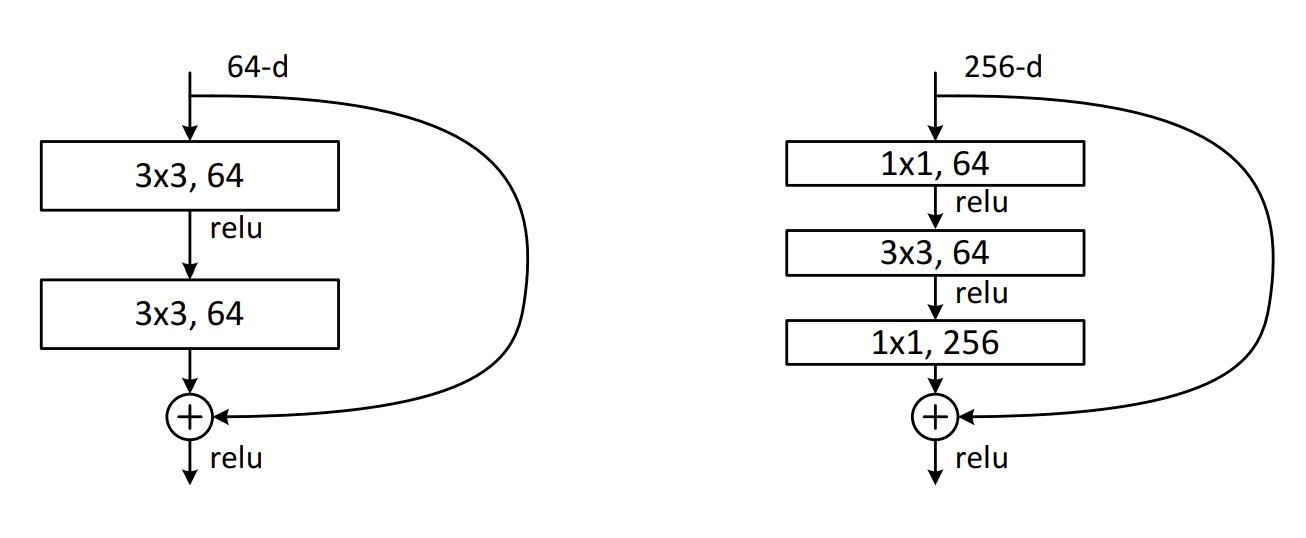
\includegraphics[width=0.4\textwidth]{./images/resnet.png}
    \caption{Comparison between standard architecture and bottleneck architecture}
    \label{fig:resnet}
\end{figure}

The authors also introduce a bottleneck architecture to reduce computational cost while maintaining performance as shown in Figure ~\ref{fig:resnet}. This replaces a two-layer $3 \times 3$ convolutional stack with a $1 \times 1$, $3 \times 3$, $1 \times 1$ structure. The first $1 \times 1$ layer reduces channel dimensionality, the $3 \times 3$ layer performs feature extraction, and the final $1 \times 1$ layer restores dimensionality \cite{resnet}. This design enables deeper and more efficient networks and may contribute to the lightweight nature of ResNet-based action recognition models.


%%=============================================================%%
%% METHODS
%%=============================================================%%


\section{Methods}\label{sec3}


\subsection{BodyPose3DNet + PoseClassificationNet}\label{subsec2}

First, BodyPose3DNet is used to extract skeletons from the 1920 RGB videos. Each skeleton sequence is output to JSON files. Next the skeleton JSON sequences were split into train/test/val with a 70/15/15 split. Importantly, the videos were split randomly by actor so that the beginners and experts were distributed into each split. Also, all three videos for each actor were placed into the same split to prevent train-test contamination. 

Once the data was processed into the correct format for PoseClassificationNet, multiple fine-tuning iterations were conducted in TAO. In total, 15 models were fine-tuned with different training parameters. The models were evaluated on their average class accuracy on the test data. 

\subsection{ActionRecognitionNet}\label{subsec2}

\begin{figure}[t]
    \centering
    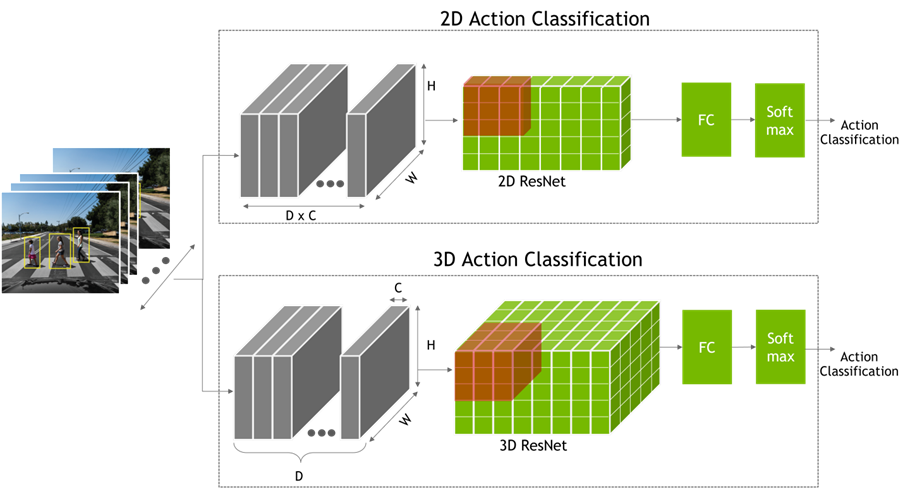
\includegraphics[width=0.8\textwidth]{./images/actionrecognitionnet-1.png}
    \caption{Diagram of the architecture of Action Recognition Net, the model can either use 3-D convolution which was what was used in this project or 2-D convolution}
    \label{fig:ARN1}
\end{figure}

Action Recognition Net’s pipeline can be broadly described as taking a video sequence as input, processing the frames into tensors, applying a ResNet backbone, and passing the resulting features through a fully connected layer and softmax to produce a class label, as illustrated in Figure~\ref{fig:ARN1}. The model supports both 2-D and 3-D ResNet backbones, however, due to the importance of temporal information for this task, the 3-D ResNet, which captures motion across frames, was used. A more detailed view of the architecture is shown in Figure~\ref{fig:ARN2}. A standard stem block first aggregates low-level features, followed by a feature extraction backbone consisting of four residual stages with increasing channel size. A regularization stage with dropout and pooling is then applied before the final classification head.

Training procedures are streamlined in the TAO toolkit, where all parameters and controls are defined in a YAML configuration file. The primary parameters modified in this work include batch size, RGB sequence length, clips per video, learning rate, decay rate, dropout, and sample rate. The input resolution was set to $224 \times 224$, which is the standard input size for ResNet-based architectures \cite{resnet} and matches the resolution used during pretraining.

Although the model operates on video sequences during inference, training requires frames extracted from videos, ordered temporally, and organized into a specific directory structure as defined in the documentation. A Python script was used to preprocess the dataset, perform an 8:1:1 train/validation/test split, and convert videos into the required frame format. The primary evaluation metrics are validation accuracy per epoch and test accuracy from evaluation on the test dataset.

\begin{figure}[t]
    \centering
    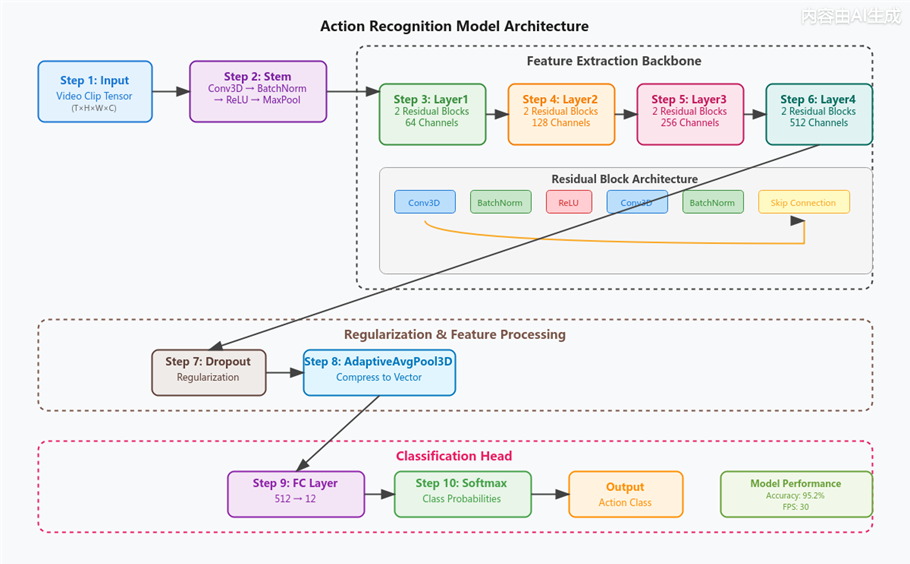
\includegraphics[width=0.8\textwidth]{./images/actionrecognitionnet-2.png}
    \caption{More detailed diagram of Action Recognition Net, diagram details each layer and broadly categorizes it into main blocks of preprocessing, feature extraction, regularization and classification}
    \label{fig:ARN2}
\end{figure}


%%=============================================================%%
%% RESULTS
%%=============================================================%%


\section{Results}\label{sec4}


\subsection{PoseClassificationNet}

\begin{table}[t]
\centering
\caption{Per-class and overall accuracy (\%) across experimental configurations.}
\label{tab:results}
\begin{tabular}{lcccc}
\toprule
\textbf{Class} & \textbf{v1.6} & \textbf{v1.7} & \textbf{v1.9} & \textbf{v2.1} \\
\midrule
Backhand (1H)    & 16.67 & 70.83 & 62.50 & 83.33 \\
Backhand (2H)    & 66.67 & 12.50 & 75.00 & 83.33 \\
Backhand Slice   & 22.22 & 20.83 & 50.00 & 58.33 \\
Backhand Volley  & 44.44 & 58.33 & 45.83 & 45.83 \\
Forehand Flat    & 83.33 & 79.17 & 87.50 & 87.50 \\
Forehand Open    & 38.89 & 75.00 & 33.33 & 75.00 \\
Forehand Slice   & 11.11 & 12.50 & 50.00 & 91.67 \\
Forehand Volley  & 77.78 & 70.83 & 45.83 & 41.67 \\
Overhead         & 11.11 & 50.00 & 29.17 & 70.83 \\
Serve Flat       & 66.67 & 25.00 & 45.83 & 33.33 \\
Serve Kick       & 22.22 & 50.00 & 50.00 & 45.83 \\
Serve Slice      & 11.11 &  0.00 &  8.33 & 33.33 \\
\midrule
\textbf{Overall} & 39.35 & 43.75 & 48.61 & \textbf{62.50} \\
\bottomrule
\end{tabular}
\vspace{2pt}
\begin{flushleft}
\footnotesize
\textit{v1.6}: subject-based split, lr=0.01. 
\textit{v1.7}: random split, lr=0.01. 
\textit{v1.9}: random split, lr=0.1. 
\textit{v2.1}: random split, lr=0.1, corrected focal length.
\end{flushleft}
\end{table}

Our best-performing model (v2.1) achieved an overall accuracy of 62.50\% on the 12-class tennis shot classification task, surpassing the best results reported in the original THETIS paper \cite{thetis}. The original authors achieved a peak of 60.23\% using STIP on the depth masks, and 57.50\% using Dense Trajectories also on the depth masks. Critically, our result is obtained entirely from RGB video --- which the original authors did not evaluate --- using a deep learning pipeline rather than hand-crafted feature extraction. The per-class and overall accuracies across all four experimental configurations are summarized in Table~\ref{tab:results}.

The progression from v1.6 to v2.1 reflects a consistent improvement in overall accuracy from 39.35\% to 62.50\%, driven by three key changes: switching from a subject-based to a random train/test split, increasing the learning rate from 0.01 to 0.1, and correcting an error in the focal length parameter used during the dataset conversion step. The focal length correction proved to be the most impactful single change, producing a jump in overall accuracy from 48.61\% in v1.9 to 62.50\% in v2.1. An incorrect focal length caused BodyPose3DNet to produce systematically distorted 3D joint positions, which the downstream ST-GCN classifier then had to learn from. Once corrected, the classifier benefited substantially without any changes to the model architecture or training procedure.

Despite the overall improvement, some classes remained challenging. Serve flat (33.33\%), serve slice (33.33\%), and forehand volley (41.67\%) continue to underperform relative to other classes. This is consistent with the observation in the original THETIS paper \cite{thetis} that certain shot types are visually very similar to one another, particularly among the serve variants, which differ primarily in subtle wrist and racket positioning.

\subsection{Action Recognition Net}\label{subsec1}

\begin{table}[t]
\centering
\setlength{\tabcolsep}{7pt}
\begin{tabular}{lccccccccc}
\toprule
Run & Acc & BS & Seq & SR & LR & DO & CPV & Decay & Ep \\
\midrule
transfer & 75.98 & 16 & 32 & 1 & 0.0015 & 0.0 & 16 & 0.1 & 30 \\

sample\_4 & 88.235 & 8 & 3 & 3 & 0.0005 & 0.10 & 8 & 0.1 & 14 \\

sample\_6 & 85.784 & 8 & 2 & 3 & 0.0005 & 0.10 & 8 & 0.1 & 14 \\

cont\_4 & 88.725 & 8 & 3 & 3 & 0.0001 & 0.10 & 8 & 0.1 & 20 \\

cont\_4\_2 & 89.706 & 8 & 3 & 3 & 0.0003 & 0.10 & 10 & 0.2 & 30 \\

cont\_4\_5 & 90.686 & 8 & 3 & 3 & 0.0002 & 0.10 & 14 & 0.2 & 35 \\
\bottomrule
\end{tabular}
\caption{Summary of runs. Acc: accuracy (\%), BS: batch size, Seq: RGB sequence length, SR: sample rate, LR: learning rate, DO: dropout, CPV: clips per video.}
\label{tab:results}
\end{table}

The results shown are a subset of all experiments, selected to highlight key parameter changes that produced significant effects. The initial run, \textit{transfer}, used default YAML parameters with pretrained weights and revealed weaknesses in three classes backhand volley, flat service, and smash with accuracies around 50\% as shown in table ~\ref{tab:per_class_results}.

The first major milestone, sample\_4, achieved a 12\% improvement in overall accuracy. This gain was primarily attributed to reducing the RGB sequence length from 32 to 3 and introducing dropout. Additionally, the validation accuracy and loss curves~\ref{fig:curve1} indicated that performance plateaued around epoch 14, suggesting that longer training was unnecessary. In this run, the weakest class was forehand slice at 76.47\%, while most other classes achieved accuracies between 80 to 90\%.

Subsequent experiments, including sample\_6, showed that an RGB sequence length of 3 was optimal, as both increasing and decreasing this value reduced performance. The run cont\_4 marked the second major milestone, surpassing the previous plateau of approximately 85\% accuracy. This improvement was attributed to initializing from the sample\_4 checkpoint, reducing the learning rate, and halving the batch size, which introduced noisier updates that helped escape the plateau.

The final runs aimed to exceed 90\% accuracy by continuing training from the best checkpoint using short training intervals (5–10 epochs), higher learning rates, and increased decay. These adjustments encouraged more aggressive learning early in training before stabilizing. This behavior is reflected in Figure~\ref{fig:curve2}, which shows more unstable accuracy and loss curves compared to the smoother trends in Figure~\ref{fig:curve1}.


\begin{table}[t]
\centering
\setlength{\tabcolsep}{5pt}
\begin{tabular}{lcccccc}
\toprule
Class & transfer & sample\_4 & sample\_6 & cont\_4 & cont\_4\_2 & cont\_4\_5 \\
\midrule
backhand & 82.35 & 88.24 & 82.35 & 88.24 & 88.24 & 88.24 \\
backhand2hands & 88.24 & 94.12 & 94.12 & 94.12 & 94.12 & 94.12 \\
backhand\_slice & 70.59 & 88.24 & 88.24 & 88.24 & 94.12 & 94.12 \\
backhand\_volley & 52.94 & 100.0 & 88.24 & 100.0 & 100 & 100.0 \\
flat\_service & 58.82 & 82.35 & 76.47 & 82.35 & 82.35 & 82.35 \\
forehand\_flat & 76.47 & 82.35 & 94.12 & 94.12 & 88.24 & 94.12 \\
forehand\_openstands & 94.12 & 100.0 & 94.12 & 100.0 & 100.0 & 100.0 \\
forehand\_slice & 94.12 & 76.47 & 82.35 & 82.35 & 76.47 & 76.47 \\
forehand\_volley & 82.35 & 94.12 & 94.12 & 88.24 & 94.12 & 94.12 \\
kick\_service & 82.35 & 82.35 & 88.24 & 88.24 & 82.35 & 88.24 \\
slice\_service & 76.47 & 88.24 & 82.35 & 88.24 & 94.12 & 94.12 \\
smash & 52.94 & 82.35 & 64.71 & 70.59 & 82.35 & 82.35 \\
\midrule
Total Accuracy & 75.98 & 88.235 & 85.784 & 88.725 & 89.706 & 90.686 \\
\bottomrule
\end{tabular}
\caption{Per-class accuracy across training runs.}
\label{tab:per_class_results}
\end{table}

\begin{figure}[t]
    \centering
    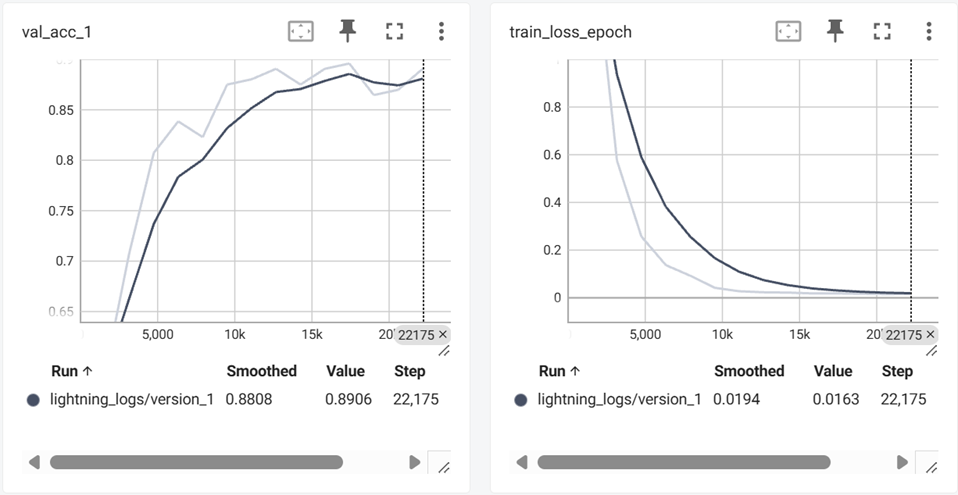
\includegraphics[width=0.8\textwidth]{./images/training-curve-exp-sample-4.png}
    \caption{Validation accuracy and training loss graphs of the run sample\_4}
    \label{fig:curve1}
\end{figure}

\begin{figure}[t]
    \centering
    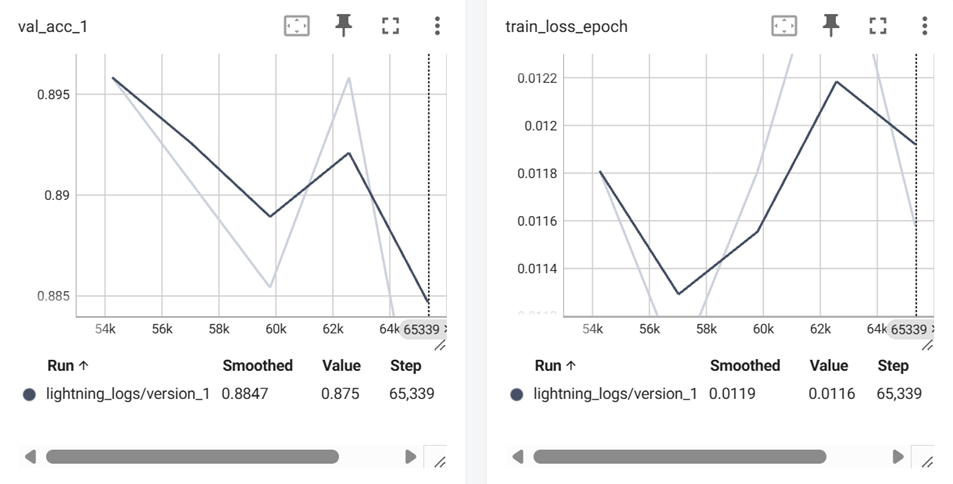
\includegraphics[width=0.8\textwidth]{./images/training-curve-best.png}
    \caption{Validation accuracy and training loss graphs of the run cont\_4\_5}
    \label{fig:curve2}
\end{figure}


%%=============================================================%%
%% DISCUSSION
%%=============================================================%%


\section{Discussion}\label{sec5}

The results for PoseClassificationNet suggest that a skeleton-based model discards important information from video sequences of tennis actions, particularly the position and movement of a tennis racket. For this reason we suggest that future researchers avoid using human skeleton graphs as the base for tennis shot classification. Instead of using human skeleton based keypoints, we suggest training a model to extract tennis keypoints that include points on the tennis racket. In order to capture the important information of a racket's position we suggest two keypoints on the racket frame (to capture its facing direction). Because the racket is essentially a flat plane, two keypoints along the frame should be sufficient. 

The results for ActionRecognitionNet indicate that the most influential parameters for effective learning were learning rate, RGB sequence length, and clips per video. Among these, RGB sequence length had the largest impact, producing the most significant increase in accuracy. This is likely because the dataset videos are relatively short (around 80–100 frames), making a sequence length of 32 too long for capturing the short, precise motion cues required for tennis action recognition.

A lower learning rate also improved performance, likely due to the difficulty of the dataset, where many actions are visually similar. A smaller learning rate may have helped the model better distinguish subtle differences between motions. Clips per video, while reduced in early runs, had a greater impact when gradually increased in later experiments. Increasing this parameter likely provided more temporal coverage and redundancy, allowing weaker classes to improve relative to stronger ones.

Although training results were strong, real-time inference using the DeepStream pipeline was less effective. Testing with both dataset videos and live webcam input suggested that the issue was not caused by preprocessing or pipeline configuration. Instead, the model appeared to struggle with generalization beyond the dataset distribution. This is supported by several dataset limitations, including its small size, standardized filming conditions, limited environments, and lack of varied perspectives.

Overall, while real-time inference was not achieved, the results demonstrate that TAO Toolkit’s lightweight models are capable of learning complex tasks such as tennis action recognition. The primary limitation appears to be the dataset rather than the model or pipeline.


%%=============================================================%%
%% CONCLUSION
%%=============================================================%%


\section{Conclusion}\label{sec6}

This work demonstrates that lightweight deep learning models trained within the NVIDIA TAO Toolkit are capable of tackling fine-grained sports action recognition, a task that has historically required hand-crafted features and specialized sensor hardware. The gap in performance between PoseClassificationNet and ActionRecognitionNet suggests that for tasks where object tracking is critical to classification --- such as tennis, where the racket is often a distinguishing feature between shots --- skeleton-based representations are fundamentally limited regardless of the quality of the underlying pose estimator. Looking forward, the ability to deploy such models in real-time via DeepStream pipelines has promising implications for sports coaching and performance analysis.


%%=============================================================%%
%% BIBLIOGRAPHY
%%=============================================================%%


\bibliography{sn-bibliography}

\end{document}
